\documentclass{llncs}

% \usepackage[letterpaper, margin=1.25in, tmargin=1.25in, bmargin=1.25in]{geometry}
%\usepackage{url}
\usepackage[T1]{fontenc}
\usepackage{float}
%\usepackage{minicaption}
\usepackage{breakurl}                  % Not needed if you use pdflatex only.
\usepackage{hyperref}
\usepackage{underscore}             % Only needed if you use pdflatex.
\usepackage[nocompress]{cite}   
\usepackage{makecell}
%\pagestyle{empty}
\usepackage{amsmath}
\usepackage{amssymb}
\usepackage{amsbsy}
% \usepackage{alltt}
\usepackage{hhline}
\usepackage{xcolor,colortbl}
\usepackage{mathpartir}
\usepackage{tikz}
\usepackage{graphicx}
\usepackage{subcaption}   % used for figures in experimental evaluation
\usepackage[ruled,vlined]{algorithm2e}
%\usepackage[linesnumbered,ruled]{algorithm2e}
\usepackage{amsmath}
%mmu algorithm
%\usepackage{algorithm}
\usepackage{algorithmic}
\usetikzlibrary{arrows,arrows.meta,calc,positioning,backgrounds,fit,shapes,shadows,trees}

\tikzset{%
  thick arrow/.style={
     -{Triangle[angle=120:1pt 1]},
     line width=1.5cm, 
     draw=teal!70
  },
  arrow label/.style={
    text=white,
    font=\sffamily\fontsize{12}{12}\selectfont,
    align=center,
    yshift=-1.25cm
  },
  set mark/.style={
    insert path={
      node [midway, arrow label, node contents=#1]
    }
  }
}

\tikzset{
  basic/.style  = {draw,rectangle,font=\sffamily\fontsize{12}{12}\selectfont}, %text width=2cm, drop shadow},
  root/.style   = {basic, font=\sffamily\fontsize{12}{12}\selectfont, rounded corners=2pt, thin, align=center,
                   fill=orange!30},
  level 0/.style = {basic, font=\sffamily\fontsize{12}{12}\selectfont, thin, align=center, fill=blue!10},
  level 1/.style = {basic, trapezium, trapezium left angle=70, trapezium right angle=110, font=\sffamily\fontsize{12}{12}\selectfont, thin, align=center, fill=green!20},
  level 2/.style = {basic, font=\sffamily\fontsize{12}{12}\selectfont, rounded corners=2pt, thin, align=left,
    fill=yellow!30},
  level 3/.style = {basic, font=\sffamily\fontsize{12}{12}\selectfont, rounded corners=2pt, thin, align=left,
    fill=blue!20, text width=12em},
  level 4/.style = {basic, font=\sffamily\fontsize{12}{12}\selectfont, thin, align=center, 
    fill=green!30},
  level 5/.style = {basic, font=\sffamily\fontsize{12}{12}\selectfont, thin, align=center, 
    fill=orange!30},
  level 6/.style = {basic, rectangle, font=\sffamily\fontsize{12}{12}\selectfont, thin, align=center, 
    fill=cyan!20},
   boxaround/.style={draw=violet, font=\sffamily\fontsize{12}{12}\selectfont, thick, dashdotted,
     inner sep=0.8em},
 >=latex
}

\usepackage{tikz}
\usetikzlibrary{arrows, positioning, shapes, fit, backgrounds}

\usepackage{paralist}
\usepackage{boxedminipage} %proof rules
\usepackage{booktabs} %proof rules

\newcommand{\imp}{\Rightarrow}
\newcommand{\etal}{\textit{et al. }}
\newcommand{\adhoc}{\textit{ad hoc}}
\newcommand{\ie}{\textit{i.e.}}
\newcommand{\etc}{\textit{etc}}
\newcommand{\eg}{\textit{e.g.}}
\newcommand{\konst}[1]{\ensuremath{\mbox{\sf{#1}}}}
\newcommand{\eps}{\varepsilon}
\newcommand{\nil}{\konst{[\,]}}
\newcommand{\cons}[2]{{#1}\boldsymbol{:}\boldsymbol{:}{#2}}
\newcommand{\hollamb}{\boldsymbol{\lambda}}
\newcommand{\itelse}[3]{\mbox{$\mbox{\tt if}\ {#1}\ \mbox{\tt then}\ {#2}\
    \mbox{\tt else}\ {#3}$}}
\newcommand{\set}[1]{\{ {#1} \}}
\newcommand{\Lang}[1]{\ensuremath{{\cal L}({#1})}}
\newcommand{\inbox}[1] {\begin{center}
                         \framebox{\parbox{0.984\textwidth}{#1}}
                         \end{center}}
\newcommand{\HOL}{\textsc{HOL}}

% for backslashes in alltt environments
\newcommand{\bs}{\texttt{\symbol{92}}}

\usepackage{scalerel}
\newcommand\sbullet[1][.6]{\mathbin{\ThisStyle{\vcenter{\hbox{%
  \scalebox{#1}{$\SavedStyle\bullet$}}}}}%
}

\DeclareMathAlphabet{\mathpzc}{OT1}{pzc}{l}{it}

%%%%%%%
%\input{../final/lib/coq-listings}

\begin{document}
%
\title{A Neuro-Symbolic Approach to Enhanced Model-Based Systems Engineering}%Towards Explainable Compositional Reasoning}%Assume-Guarantee Reasoning Environment Copilot (AGREE-Dog)}
%
%\titlerunning{Assume-Guarantee Reasoning Environment Copilot (AGREE-Dog)}
% If the paper title is too long for the running head, you can set
% an abbreviated paper title here
%
\author{Amer Tahat\and
  Isaac Aumundson \and
  David Hardin \and
  Darren Cofer}
%
\authorrunning{A. Tahat et al.}
% First names are abbreviated in the running head.
% If there are more than two authors, 'et al.' is used.
%
\institute{Collins Aerospace\\ Cedar Rapids, IA 52498  USA\\
  \email{\{amer.tahat, isaac.aumndson, david.hardin, daren.cofer\}@collins.com}
%\and Institute for Information Sciences \\ The
%  University of Kansas \\ Lawrence, KS 66045  USA\\
 % \email{\{ampetz,palexand\}@ku.edu}
  }
%

%%%%%%%%
\maketitle

\begin{abstract}
Formal verification tools like model checkers have long demonstrated their capability to ensure mission-critical properties are satisfied, yet their adoption in the aerospace and defense industries remains limited. Surveys consistently identify difficulty in interpreting analysis results, especially counterexamples, as a primary barrier. Previously, our team developed AGREE, an assume-guarantee compositional reasoning tool for architectural models, which generates detailed but often challenging-to-interpret counterexamples.
%
In this paper, we introduce AGREE-Dog, an open-source generative AI copilot integrated into the OSATE IDE to enhance explainable compositional reasoning with AGREE and AADL. AGREE-Dog automates 16 DevOps and ProofOps steps, utilizing a novel context-selection and memory management system to efficiently manage evolving artifacts and historical interactions.
%
We introduce structural and temporal metrics to evaluate the typically overlooked human contributions in generative AI-supported workflows. Evaluations using 13 UV fault-injection scenarios demonstrate a significant reduction in manual effort (less than 0.1\,\% of tokens authored by users), rapid convergence of counterexample repairs (84.6\,\% resolved in a single iteration, accuracy increasing to about 92\,\% after two iterations, and reaching 100\,\% within three iterations), and low latency (average LLM response under 22 seconds, with negligible AGREE-Dog computational overhead). We also discuss limitations and future work. These promising results motivate further exploration into explainable model-based systems engineering (MBSE).
\keywords{LLM \and Formal verification \and MBSE \and AGREE \and AADL \and Compositional reasoning}
\end{abstract}

\section{Introduction}
\label{sec:introduction}
%-----------------------
%\section{Introduction}
%-----------------------
Formal methods provide a mathematically rigorous means of verifying correctness in high-assurance systems, such as those used in the aerospace and defense industries. Certification guidance such as DO-333~\cite{DO-333} explicitly outlines how formal methods can meet airworthiness objectives for commercial aircraft software. Despite their proven effectiveness, adoption within traditional development workflows remains limited, hampered by scalability challenges, poorly designed tooling, and significant barriers to entry due to specialized training requirements~\cite{davis-fmics13}.

The DARPA Pipelined Reasoning of Verifiers Enabling Robust Systems (PRO-VERS) program was launched to address these adoption barriers by developing scalable, human-centered formal verification workflows that seamlessly integrate into existing aerospace and defense engineering practices. Central to PROVERS' objectives is enabling usability even among engineers who lack extensive formal methods expertise, thereby fostering broader adoption and enhancing system dependability.

In response, our team has developed the Industrial-Scale Proof Engineering for Critical Trustworthy Applications (INSPECTA) framework~\cite{inspecta}. INSPECTA comprises two integrated layers—\textit{ProofOps} and \textit{DevOps}—that embed formal verification directly into modern DevOps pipelines. The framework emphasizes scalability and explainability as primary design objectives, aligning closely with the PROVERS program’s goals.

Within INSPECTA’s \textit{ProofOps} workflow, we employ the Assume-Guarantee Reasoning Environment (AGREE)\cite{compositional-analysis-agree}, a compositional verification tool designed specifically for the Architecture Analysis and Design Language (AADL)~\cite{feiler-aadl}.
%
Although AGREE avoids many of the scalability pitfalls found in monolithic verification tools, its counterexample outputs remain difficult to interpret. Like many model checkers, AGREE produces tabular counterexamples that trace the state of variables across multiple time steps. These can involve intricate temporal logic, nested states, and violations spanning architectural layers, posing challenges even for experienced engineers~\cite{cex-explanation}. The diagnostic and repair process may span, hours, days, or weeks for large, evolving models based on user experties.

Recently, generative AI, and particularly large language models (LLMs), have shown promising potential to improve explainability and guide automated formal verification and counterexample repair. Early efforts include OpenAI’s GPT-f, which achieved notable success in Metamath theorem proving~\cite{polu2020generative, megill2019metamath}. Other initiatives have applied LLMs successfully to proof repair in Isabelle/HOL~\cite{first2023baldur}, theorem diagnosis in Coq~\cite{zhang2023getting}, and discovering program invariants~\cite{pei2023can, wu2023lemur}. Stanford and VMware’s Clover project represents another significant step forward, focusing on verifiable code generation with generative assistance~\cite{sun2024clover}. Tahat et al. demonstrated high success rates using multi-turn conversational LLMs for proof repair in Coq, underscoring conversational learning’s value in formal reasoning domains~\cite{CoqDog, CoqDogHCSS24}.
%
Apple's GSM-Symbolic~\cite{mirzadeh2025gsmsymbolic} highlighted fundamental limitations of LLMs in symbolic reasoning tasks. Similarly, Amazon’s recent SMT-backed hallucination prevention framework~\cite{amazon2024mathematical}, while innovative, remains closed-source, available exclusively as a web service, and has yet to integrate within aerospace-specific MBSE pipelines such as those based on AADL.

In this paper, we introduce AGREE-Dog, an open-source generative AI copilot integrated directly into the OSATE IDE. AGREE-Dog is purpose-built to support explainable, compositional reasoning within MBSE workflows, particularly targeting aerospace and defense applications using AADL and AGREE. It automates 16 DevOps and ProofOps steps, including requirements ingestion, context-aware prompt construction, semantic diffing, formal validation, and log analysis. Notably, AGREE-Dog employs a specialized conversational memory management and context-selection approach that efficiently represents evolving verification artifacts in a concise, fixed-size token window, dramatically simplifying the complexity inherent in tracking and repairing system-level contract violations (see Section~\ref{sec:key-impact} %and Appendix~\ref{appendix:test-scenarios} 
for detailed evaluation and artifact descriptions).

To quantify these benefits, we introduce novel structural and temporal evaluation metrics, explicitly addressing aspects such as repair convergence, human intervention level, token efficiency, and response latency.

The rest of this paper is organized as follows. 
Section~\ref{sec:design-architecture} presents AGREE-Dog’s architecture and orchestration strategy. Section~\ref{sec:key-impact} details our experimental evaluation and findings. We conclude with current limitations and outline future work aimed at enhancing autonomy and generalization across verification domains.




\section{Explainable AGREE}
\label{sec:Explainable-AGREE}
\subsection{Overview}
%\subsection{Overview}
\label{Overview}
AGREE provides a formal contract language for specifying \textit{assumptions} (i.e., expectations on a component's input and the environment) and \textit{guarantees} (i.e., bounds on a component's behavior).  Because AGREE is implemented as an AADL \textit{annex} in the Open Source AADL Tool Environment (OSATE), the contracts are specified directly on components in the AADL model.  AGREE then uses a k-induction model checker to prove properties about one layer of the architecture using properties allocated to subcomponents. The analysis proves correctness of (1) component interfaces, such that the output guarantees of each component must be strong enough to satisfy the input assumptions of downstream components, and (2) component implementations, such that the input assumptions of a system along with the output guarantees of its sub-components must be strong enough to satisfy its output guarantees.

When a contract violation is found (i.e., when an assumption is determined to be invalid or a guarantee is unsupported), AGREE produces a counterexample consisting of values for each system variable at each execution step.  A sample counterexample is depicted in Figure~\ref{fig:cex}.  Currently, OSATE includes the AADL Simulator tool that can accept an AGREE counterexample as input and walk through the trace in the graphical editor, but it is of limited help when it comes to identifying the root cause of the contract violation.


\begin{figure}[t] 
	\centering 
\includegraphics[height=0.6\textwidth, width=0.9\textwidth]{cex.png}
	\caption{AGREE counterexample generated from the \texttt{Car} model.}
	\label{fig:cex} 
\end{figure}

%\subsection{Making Counterexamples Actionable} 
We therefore desire AGREE counterexamples that are \textit{actionable}; that is, an explanation of the violation in terms that will quickly lead to a passing analysis (e.g., by making changes to the model or formal contract).
%
%In the following sections, we introduce AGREE-Dog, 
To achieve this, we implemented
an interactive conversational copilot powered by GPT-4o (omni) multi-modal generative AI, specifically developed to assist AGREE users in identifying the root causes of counterexamples and to support the subsequent model repair process. It was designed to be user-friendly and integrates with the OSATE IDE (see Figure~\ref{fig:AGREEDOG}). 
%\footnote{In Figure~\ref{fig:AGREEDOG} AGREE-Dog is a specific instance of the INSPECTA-Dog toolset, where users can select the copilot's identity. This paper focuses on the AGREE-Dog instance, while other instances of INSPECTA-Dog are beyond the scope of this discussion.}

In the remainder of this paper, we detail our methodology and present our key findings using the \texttt{Integer\_Toy} and \texttt{Car} models included with the AGREE distribution.

\begin{figure*}[t]  
    \centering
    \includegraphics[height=0.6\textwidth, width=1.0\textwidth]{AGREE-DOG-high-rs.png}%AGREE-Dog.png}  
%    \caption{AGREE-Dog, acting as a copilot to OSATE, provides explanations for the counterexample generated by the AGREE tool for the AADL model \texttt{Car.aadl}.}
    \caption{AGREE copilot in OSATE provides an explanation for a counterexample generated on the \texttt{Car} model.}
    \label{fig:AGREEDOG}
\end{figure*}


 %In the remainder of this section, we detail our methodology, for addressing the primary challenges we have encountered, present our key findings, and discuss the current limitations and directions for future work. To elucidate these challenges, we use the \texttt{Toy\_Integer} and \texttt{Car} models included with the AGREE distribution as two running examples throughout the paper.

\section{Problems and Core Bottelnecks}
\subsection{Contextual Prompt Constraints Problem}

The GPT-4o generative multi-modal model exhibits significant power in translating human instructions into code and vice versa, particularly when the language in question has been part of its pre-training data and there exists a substantial open-source code base, such as C or Python. However, this capability comes with the drawback of potential hallucinations. Since AGREE is not as widely adopted as languages like C or Python, this problem is exacerbated. 
%Consequently, one of the primary challenges we encountered involved the explainability of counterexamples due to the absence of relevant context.
Consequently, the lack of relevant context is a significant challenge for generating explainable AGREE counterexamples. 

%\subsubsection{AGREE-Dog Retrieval-Augmented Generation (RAG) System}
% To mitigate the Contextual Prompt Constraints problem we designed AGREE-Dog RAG system we implemented the system to be dynamic, allowing it to adjust its context based on user inquiries. 
To mitigate the contextual prompt constraints problem, we implemented a dynamic Retrieval-Augmented Generation (RAG) system, allowing it to adjust its context based on user inquiries.

Despite GPT-4o's 128k token capacity, which we estimate can accommodate several thousand lines of AADL in a single prompt, uploading an entire repository's contents can be prohibitively expensive and may well exceed the prompt token limitations. We therefore implemented a practical two-step optimization technique to meet our current needs.

First, the RAG system reads the top-level AADL file.  It then parses the file's import chain, extracting only the files in the model workspace that are specified on this chain. This step significantly reduces the initial prompt size. %, see Figure \ref{fig:AGREEDOG}.  
%
The second optimization addresses another practical requirement: handling parts of the repository that may have been included in the model's pre-training data, such as core libraries. To manage this, the RAG system applies a filtering technique to the file names, guiding the system to ignore certain files, such as standard libraries, and retain user-defined files. This approach further reduces the initial prompt size to include only files that the model has not previously encountered. Finally, user inputs are automatically incorporated into the extracted context from the current file and its import chain, allowing for more accurate responses to user inquiries.

This approach significantly mitigates contextual constraint-based hallucinations that can arise from the absence of AADL model specifications. However, it does not address the absence of the counterexample itself or the lack of guidance on the critical system requirements that should be preserved during the model repair process.
 

\subsection{Model Repair Problem}

Given that counterexamples are generated interactively and may not be included in the initial context, we dynamically extend the RAG system. This allows users to upload an exemplar AADL/AGREE model along with a corresponding counterexample (in text or CSV format). %(Figure \ref{fig:AGREEDOG2}).
Upon submission, the copilot provides a detailed, step-by-step explanation of the counterexample, identifies its root cause(s), and suggests potential solutions, as shown in Figure~\ref{fig:AGREEDOG}. 


However, a significant challenge encountered was that these explanations and suggested alternatives could include two types of hallucinations, both syntactic and semantic. The former are typically minor and can be detected and resolved using a multi-shot approach. The latter are more problematic, as the copilot might suggest altering a component's guarantee, which could successfully remove the counterexample but risk violating core system requirements that should remain unchanged.  We refer to this as the \textit{Model Repair Problem}. 


\subsubsection{Requirements for Counterexample Explanations}

To mitigate the Model Repair Problem, we configured the tool to generate solutions that conform to a predefined set of system requirements written in natural language, which are uploaded via a CSV file or directly included in the context. 

\begin{figure}[t]  
    \centering
    \includegraphics[width=0.8\textwidth]{REQ-AWARE-REF-high-res.png}  
    \caption{Refined explanation using a requirements file for the \texttt{Integer\_Toy} model.}
    \label{fig:REQ-AWARE-EXPL}
\end{figure}


As a result, the tool was able to more accurately identify the root cause and suggest appropriate solutions, as demonstrated in Figure~\ref{fig:REQ-AWARE-EXPL}.
%
This refinement significantly enhanced the accuracy of the recommendations.

\begin{figure*}[t]  
    \centering
    \includegraphics[height=0.6\textwidth, width=1.0\textwidth]{woof-pic-6.png}%woofpic-2 is best so far}  
    \caption{AGREE-Dog copilot repair cycle for a UV \texttt{Car} model. The left pane shows AADL contracts and successful AGREE verification; the right pane displays the copilot interface with token usage, LLM latency (32.29s), and interactive log traces. User input, feedback, and commit actions are handled through a push-button interface tightly integrated with OSATE and AGREE. This integration enables the prompt constructor and update agent to respond to proof outcomes in real time. Timestamps indicate low human turnaround and negligible orchestration overhead (sub-second per step), demonstrating effective usability and latency for interactive formal repair.}
    \label{fig:Woof}
\end{figure*}

\subsection{AGREE log and System Validity Guarantees}
\begin{figure*}[t]  
    \centering
    \includegraphics[height=0.6\textwidth,width=\textwidth]{AGREE-DOG-high-rs.png}%AGREE-Dog.png}  
    \caption{AGREE copilot in OSATE provides an explanation for a counterexample generated on the \texttt{Car} model.}
    \label{fig:AGREEDOG}
\end{figure*}
\subsection{Bidirectional Feedback Loops Operations}
\subsection{Tracibility: Copilot Log Files}
\subsubsection{LLM Latency and Human Return Time}

\subsection{Conversational Quality Assessment Problem}
\begin{figure}[htbp]
\centering % Still centering the figure
\hspace*{-1cm} % Shift the entire figure to the left by 1 cm
\resizebox{0.95\columnwidth}{!}{ % Keep the size slightly below the full column width for better fit
\tikzstyle{root} = [rectangle, fill=white!3, text width=4.5em, text centered, minimum height=2em, node distance=.10cm]
\tikzstyle{block} = [rectangle, draw, fill=blue!3, text width=5.3em, text centered, minimum height=2em, node distance=.40cm]
\tikzstyle{block1} = [rectangle, draw, fill=red!3, text width=7em, text centered, minimum height=2em, node distance=.5cm]
\tikzstyle{block2} = [rectangle, draw, fill=gray!3, text width=6em, text centered, minimum height=2em, node distance=.5cm]
\tikzstyle{block3} = [rectangle, draw, fill=green!10, text width=8em, text centered, minimum height=2em, node distance=.55cm]
\tikzstyle{line} = [draw, -latex']

\begin{tikzpicture}[auto, node distance=2cm,>=latex']
    % Place nodes
    \node [root] (root1) {};
    \node [block1, right=of root1] (interactions) {\texttt{\textbf{AGREE-Dog}} User-System Interactions};
    \node [block2, below=of interactions] (history) {Recording Metrics Automatically};
    \node [block2, right=of history] (lemma) {Model-Repair Log Files};
    \node [block2, right=of lemma] (quality) {Conversation History Management};
    \node [block3, above=of quality] (stat) {\textcolor{blue}{Statistical Analysis and Visualization}};

    % Draw edges
    \path [line] (root1)  (interactions);
    \path [line] (interactions) -- (history);
    \path [line] (history) -- (lemma);
    \path [line] (lemma) -- (quality);
    \path [line] (quality) -- (stat);
\end{tikzpicture}
} % End of resizebox
\caption{AGREE-Dog conversation quality assessment evaluation workflow.}
\label{fig:CQAS}
\end{figure}
%\subsection{Preliminary Results and Conversational Quality Assessment Problem}
 
%Our initial evaluations were conducted manually, focusing on the %copilot's ability to accurately identify the root cause of the %counterexamples, repair the model, and ensure compliance with the %requirements. The system was evaluated on two case studies. The %first case study involved the \texttt{Integer\_Toy} model, while %the second dealt with a larger model that imports several files, %totaling 7 files and approximately \texttt{380} lines of AADL. The %copilot successfully identified the root cause of all %counterexamples for the specified guarantees (13 out of 13) on the %first attempt, demonstrating a high degree of accuracy.
%%
%However, these manual evaluations highlight the need for greater %automation; consequently, we plan to develop a more automated %evaluation system to enable testing on more realistic and complex %use cases.
%, following the workflow shown in Figure~\ref{fig:CQAS}.
 



%We are in the process of selecting a golden set of examples from a formally verified library we developed previously, and constructing a testing set by introducing deliberate violations. These examples will be used by the copilot to evaluate its ability to correctly identify the root causes. While we have demonstrated initial success in this area, model repair remains a more complex challenge. This is because repairing models can result in multiple solutions, particularly for more intricate use cases. One of the key limitations is the tool's ability to consistently remove counterexamples while ensuring compliance with the specified requirements. To address these issues, we are developing a toolset aimed at measuring convergence towards the correct semantics of the golden examples, within a few-shot learning context. This remains an ongoing challenge that we will address in our future work. %extend our prior research from the \cite{coqDog} paper to improve AGREE-Dog's performance in these areas


%\subsection{Preliminary Results}








\subsection{Making Counterexamples Actionable}
\label{sec:actionable}
%\section{Making Counterexamples Actionable}
\label{sec:actionable}
We therefore desire AGREE counterexamples that are \textit{actionable}; that is, an explanation of the violation in terms that will quickly lead to a passing analysis (e.g., by making changes to the formal contract or model).
%
%In the following sections, we introduce AGREE-Dog, 
To achieve this, we implemented an interactive conversational copilot (AGREE-Dog) powered by GPT-4o and O3 multimodal generative AI models. It is specifically designed to assist AGREE users in identifying the root causes of counterexamples and applying targeted modifications during the model repair process, significantly reducing the turnaround time between verification attempts. The copilot is user-friendly and integrates seamlessly with the OSATE\,2 IDE (see Figure~\ref{fig:AGREEDOG}).

\begin{figure*}[t]
\centering
\includegraphics[height=0.6\textwidth, width=1.0\textwidth]{AGREE-DOG-high-rs.png}
\caption{AGREE-Dog copilot integrated within OSATE, providing an actionable explanation of a counterexample generated from the \texttt{Car} model.}
\label{fig:AGREEDOG}
\end{figure*}

In the remainder of this paper, we explore the motivations that drove the development of AGREE-Dog, describe its key architectural features, and evaluate its effectiveness within representative modeling and verification workflows.



\section{Motivations and Core Challenges}
\label{sec:motivations-core-challenges}
%\Section 3: Design
%\section{Motivation and Design}
%Section 3: Motivations and Core Challenges
Drawing upon our practical experience integrating AGREE within MBSE workflows, in this section we highlight central challenges and key design principles that guided the development of our LLM-based solution for generating actionable counterexample explanations and facilitating automated model repairs.

\subsection{Context-Aware Prompt Construction}
AGREE-generated counterexamples typically involve numerous variables, intricate execution traces, and extensive AADL architectural data. Incorporating detailed LLM-generated code explanations and diagnostics exacerbates this challenge. Presenting these details directly to a generative AI model without careful management %often exceeds context limitations, resulting in poor or misleading responses. 
often result in excessive context size, increasing latency, hallucinations, costs, and potentially exceeding token limits.
The key challenge is identifying and selecting only the most relevant context to include in prompts, ensuring accurate, concise explanations and actionable recommendations.

\subsection{Ensuring Validity of Automated Repairs}
Generative models might propose repairs that, while plausible, could unintentionally violate established architectural interfaces or critical system properties. Maintaining consistency within compositional reasoning frameworks, such as AGREE, requires continuous validation. Thus, repairs must be tightly integrated with formal verification steps to ensure that each modification preserves overall system correctness.

\subsection{Minimizing User Effort and Interaction Latency}
Manually reviewing detailed logs and deeply nested temporal logic from counterexamples is both error-prone and time-consuming. An effective repair process must significantly reduce user overhead by automating log analysis, semantic comparisons between successive runs, and managing formal proof re-validation. Minimizing both system latency and human interaction time is essential to achieve an efficient, near-interactive model repair workflow.

%%%%%%%%%%%%%%

\begin{figure}[t]
  \centering
  \includegraphics[width=\linewidth]{woof-pic-6.png}
  \caption{AGREE-Dog UI interface showing integrated model diagnostics, user input, token count, response time, and push-button feedback loop. Each repair cycle is proof-aware and synchronized with AGREE log results.}
  \label{fig:copilot-ui}
\end{figure}
%\label{sec:agreedog-design}
%%\section{AGREE-Dog Design}
\label{sec:agreedog-design}


\section{AGREE-Dog Architecture}
\label{sec:design-architecture}
%\section{AGREE-Dog Architecture}
\label{sec:design-architecture}

This section details AGREE-Dog’s architecture (Figure~\ref{fig:agree-dog-refined-workflow}), systematically highlighting key subsystems designed to overcome the practical challenges identified previously (Section 3). 
%
Specifically, in this section, we present AGREE-Dog’s intuitive user interface, sophisticated memory and context management algorithms, formal validation-driven feedback loops, and integration with OSATE\,2 and version control systems.

\begin{figure}[tbp]
\centering
\resizebox{0.97\textwidth}{!}{
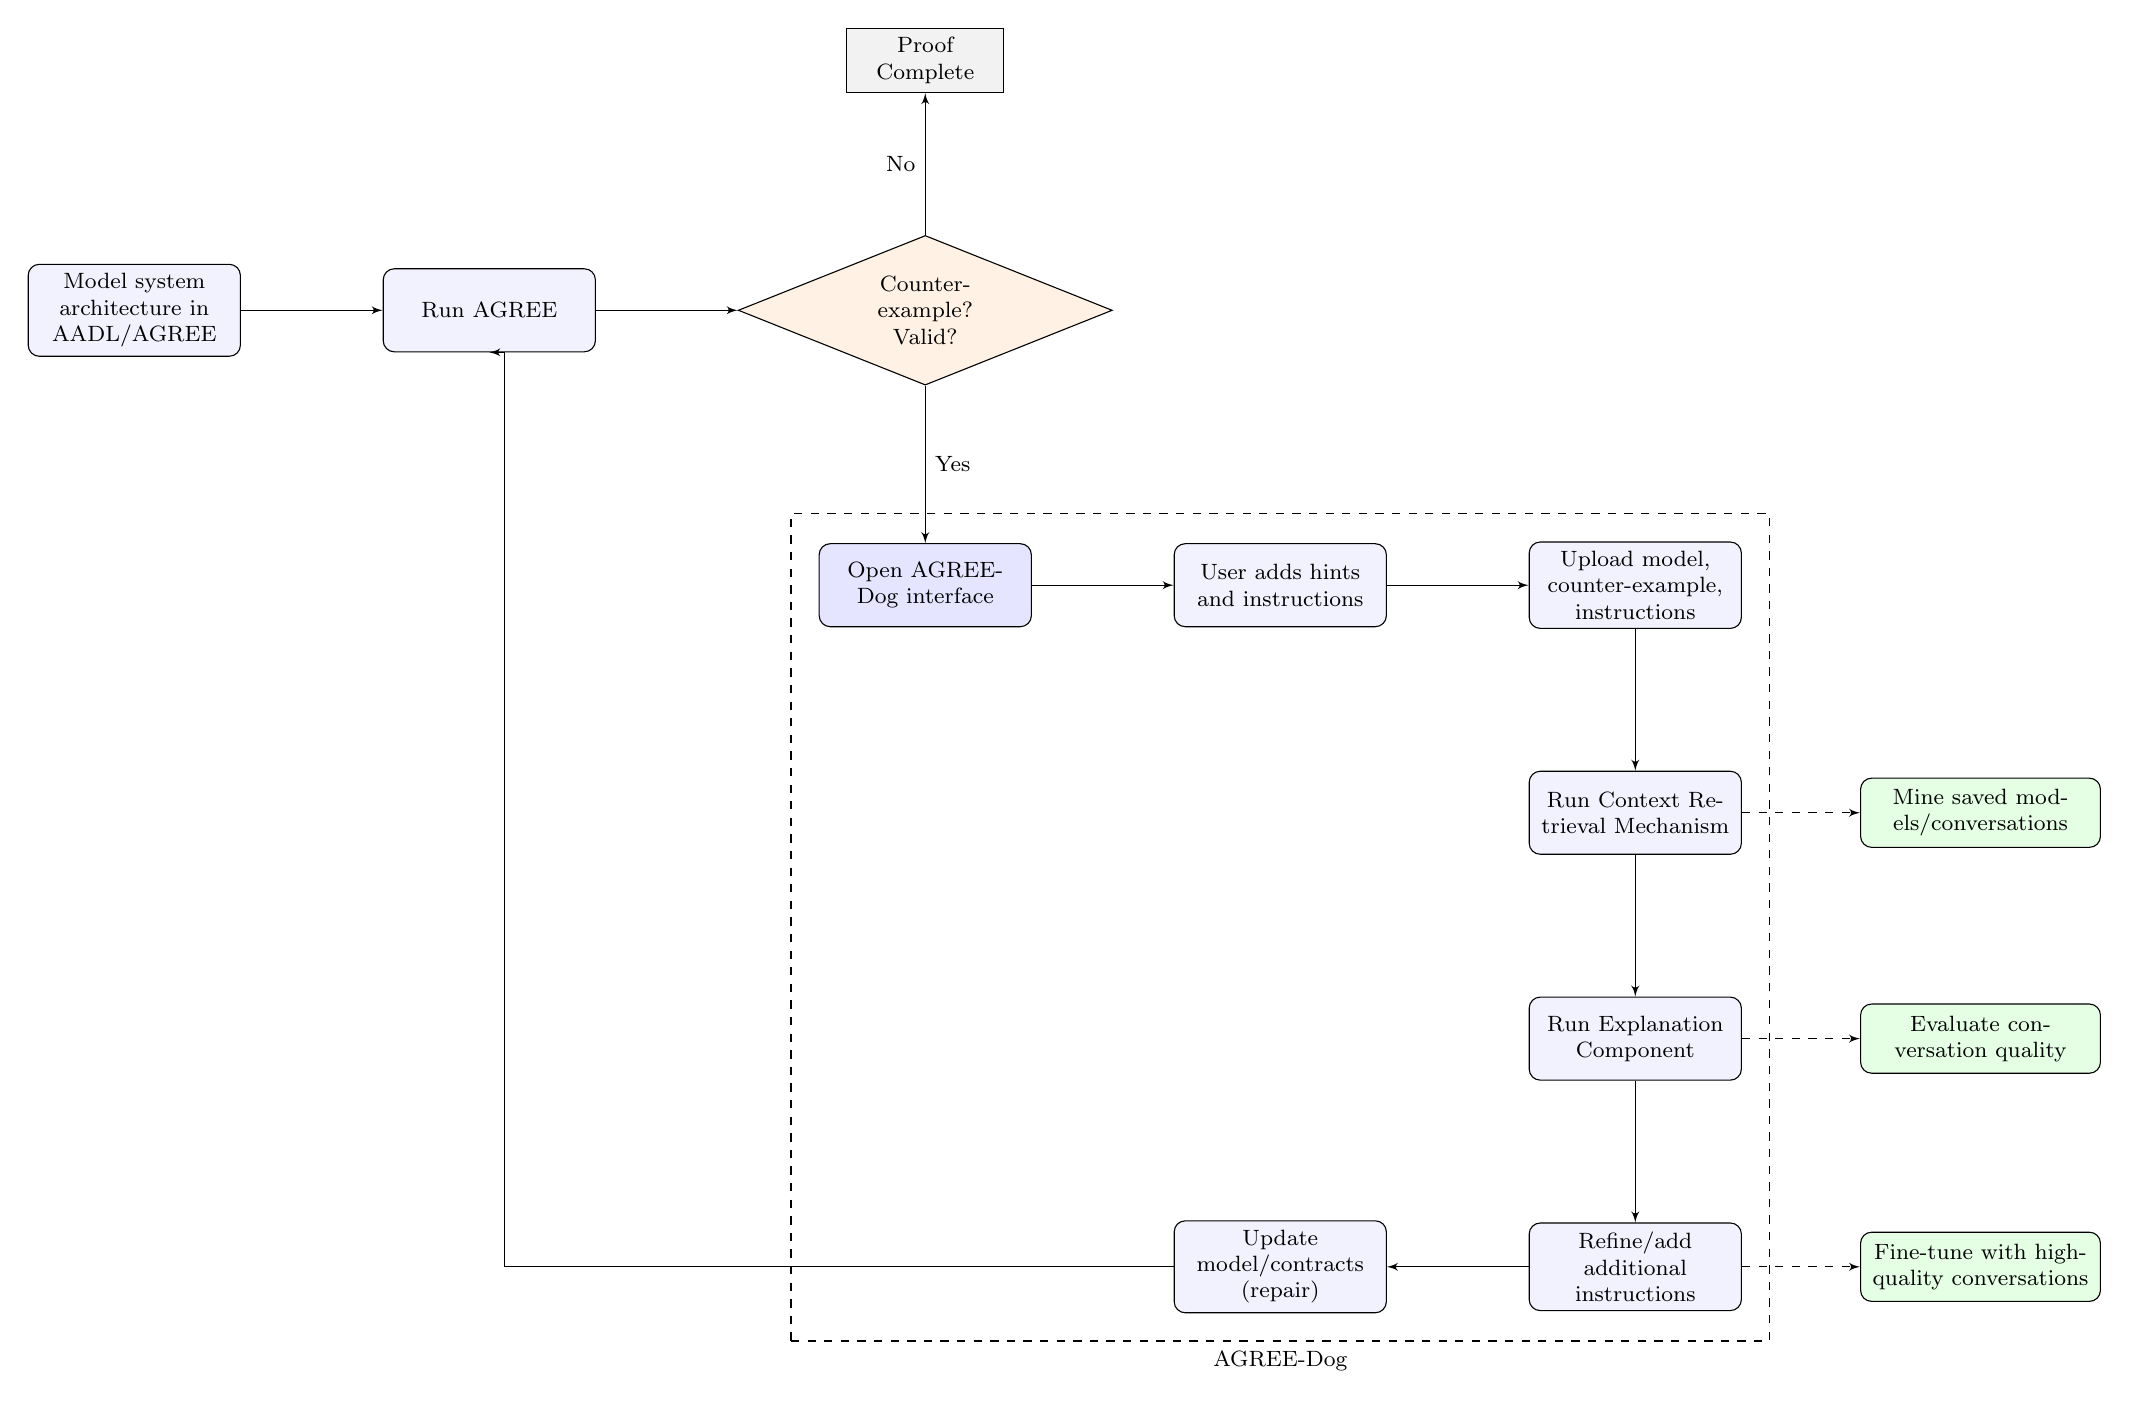
\begin{tikzpicture}[auto, node distance=1.8cm,>=latex', font=\footnotesize,
block/.style={rectangle, draw, rounded corners, fill=blue!5, text width=7em, text centered, minimum height=3em},
decision/.style={diamond, draw, fill=orange!10, aspect=2.5, inner sep=2pt, text width=6em, text centered},
result/.style={rectangle, draw, fill=gray!10, text width=5em, align=center},
annotation/.style={rectangle, draw, fill=green!10, text width=8em, align=center, minimum height=2.5em, rounded corners},
line/.style={draw, -latex'}]

% Nodes
\node[block] (model) {Model system architecture in AADL/AGREE};
\node[block, right=of model] (agree) {Run AGREE};
\node[decision, right=of agree, node distance=2.5cm] (valid) {Counter-example? Valid?};

\node[result, above=of valid] (proof) {Proof Complete};

\node[block, below=2cm of valid, fill=blue!10] (interface) {Open AGREE-Dog interface};

\node[block, right=of interface, node distance=3cm] (hints) {User adds hints and instructions};

\node[block, right=of hints, node distance=3cm] (upload) {Upload model, counter-example, instructions};

\node[block, below=of upload] (context) {Run Context Retrieval Mechanism};

\node[block, below=of context] (explain) {Run Explanation Component};

\node[block, below=of explain] (refine) {Refine/add additional instructions};

\node[block, left=of refine, node distance=4cm] (update) {Update model/contracts (repair)};

% Annotations
\node[annotation, right=1.5cm of context] (anno1) {Mine saved models/conversations};
\node[annotation, right=1.5cm of explain] (anno2) {Evaluate conversation quality};
\node[annotation, right=1.5cm of refine] (anno3) {Fine-tune with high-quality conversations};

% Paths
\path[line] (model) -- (agree);
\path[line] (agree) -- (valid);
\path[line] (valid) -- node {No} (proof);
\path[line] (valid) -- node {Yes} (interface);
\path[line] (interface) -- (hints);
\path[line] (hints) -- (upload);
\path[line] (upload) -- (context);
\path[line] (context) -- (explain);
\path[line] (explain) -- (refine);
\path[line] (refine) -- (update);

% Adjusted Loop Path from Update to Run AGREE
\path[line] (update.west) -- ++(-8.5,0,0) |- (agree.south);

% Annotation paths
\path[line, dashed] (context) -- (anno1);
\path[line, dashed] (explain) -- (anno2);
\path[line, dashed] (refine) -- (anno3);

% Enclosing box
\node[draw, dashed, inner sep=10pt, label={[align=center]below:AGREE-Dog}] 
  (box) [fit=(interface)(hints)(upload)(context)(explain)(refine)(update)] {};
\end{tikzpicture}
}
\caption{AGREE-Dog workflow illustrating the integration of formal verification with context-aware explanation and iterative model repair. %Upon detecting a valid counterexample from AGREE, the copilot interface is launched, enabling users to upload relevant artifacts and provide instructions. Context retrieval and explanation components are then invoked, guiding the refinement or repair of the model untill system wide validty is reached. The system supports both interactive user input and retrieval of prior conversations, facilitating high-quality, low-latency updates to the design under verification.
}
\label{fig:agree-dog-refined-workflow}
\end{figure}






\subsection{User Interface and Interaction Workflow}
AGREE-Dog features an intuitive, streamlined user interface (UI), (Figure~\ref{fig:copilot-ui}), seamlessly integrated within the OSATE environment, designed specifically to minimize cognitive load and simplify complex verification tasks. Central to its usability are clearly labeled, push-button controls, enabling users to directly interact with counterexample explanations, formal validations, and system-level model repairs from a single coherent point of interaction.

A fundamental design principle of this UI is to balance transparency with abstraction—clearly presenting operational outcomes without burdening users with underlying complexities. This approach promotes efficiency, productivity, and verification effectiveness.

At the center of user interaction is the \textit{Feedback} button, which synchronizes the internal state of OSATE\,2 with AGREE-Dog, updating its variables and internal data structures. This synchronization ensures coherence between AGREE-Dog's conversational state and the current OSATE\,2 project status, thus setting the stage for effective model analysis and refinement—detailed further in the next sections.%sequel.
%

We complement this mechanism, with the \textit{Insert} button which enables seamless integration of AGREE-Dog’s suggested model repairs directly into OSATE\,2,
significantly streamlining what would otherwise be a tedious manual integration process.
%
User-driven requests or specific instructions are submitted via the \textit{Submit} button and can be further elaborated upon through an integrated conversational chat window. This conversational approach encourages precise, targeted refinements by enabling iterative and detailed guidance from the user.


Additional UI elements enhance interaction quality and knowledge retention. The \textit{Save} button allows users to archive conversational histories for later review or further analysis and evaluations, as shown in Section~\ref{sec:key-impact}, while the integrated \textit{Git} control provides mechanisms for persistent storage, sharing of verification outcomes, and collaborative insight generation. 

Moreover, advanced configurations are accessible via the dedicated \textit{Settings} menu, %AT: ToDo to add Fig here or in the appendix
allowing users to customize interaction workflows and select optimal LLM models tailored to specific tasks, such as explanation and inspection using GPT-O3, or rapid code repair through the Inspection and Code Repair agents powered by GPT-O3 and GPT-4o, respectively, as detailed further in Section~\ref{sec:workflow}.

\subsection{Backend Function Call Graph and Workflow Automation}
\label{sec:workflow}

To support interactive workflows, AGREE-Dog automates 16 critical DevOps and ProofOps steps. The backend orchestration, summarized in Figure~\ref{fig:callgraph}, manages operations ranging from artifact selection and prompt construction to automated AGREE invocations. AGREE-Dog utilizes context and history-aware agents that dynamically select relevant artifacts, perform semantic diffs, and invoke proof engines. Each backend operation is highly optimized, incurring negligible runtime overhead (less than one second per operation), as demonstrated by the empirical results in Section~\ref{sec:key-impact}.


\subsection{Context Selection and Memory Management Optimization}

Effective context selection and memory management are critical to AGREE-Dog’s ability to provide precise explanations and actionable repairs involving complex AADL artifacts, execution traces, and user instructions. Addressing these challenges requires the sophisticated, carefully optimized mechanisms embedded within AGREE-Dog’s core copilot algorithm.

\subsubsection{Core Copilot Algorithm}
\textbf{Algorithm~\ref{alg:agreedog}} embodies the central context management strategy of AGREE-Dog, as conceptually outlined in Figure~\ref{fig:agree-dog-refined-workflow}. This algorithm integrates intelligent conversational state tracking, dynamic artifact selection, and optimized memory management processes to efficiently support model verification and repair tasks.

\paragraph{Optimized Dynamic Context Retrieval and Updates.}
\textbf{Algorithm~\ref{alg:agreedog}} dynamically selects a minimal yet sufficient context—including relevant AADL source files, counterexamples, AGREE logs, and system requirements, and interactive user instructions—for accurate verification and effective repair interactions. Leveraging its integrated dynamic Context Retrieval component, the algorithm selectively imports only the most recently updated model artifacts, identified through AGREE-log updates received from OSATE\,2, by traversing dependency chains and referencing stored conversational data.

By default, the context retrieval strategy excludes standard training data such as core libraries typically present in LLM training sets, thus optimizing token usage. However, users retain flexibility to explicitly include or exclude any files from the complete import chain during initialization, incorporating selected context elements into the initial prompt. Once included, these explicitly imported files remain static in memory unless updated explicitly by the user or signaled via AGREE logs. Additionally, natural-language requirement files (e.g., CSV-based inputs), not tracked by AGREE logs, are monitored independently with automatic checks performed every two seconds to detect changes.

This nuero-sympolic (intersymbolic) and user-customizable selection process significantly reduces redundancy, enhances convergence speed toward correct model solutions, minimizes generative model latency, and mitigates hallucinations caused by irrelevant context.

%\section algorithm 
\begin{algorithm}[htbp]
\caption{AGREE-Dog Interactive Copilot Prompt Construction and Counterexample Handling}
\label{alg:agreedog}
\KwIn{AADL Model Files, Counterexample File (optional), System Requirements (optional)}
\KwOut{Prompt for GPT-based AGREE-Dog Copilot, Actionable Repair Suggestions}

\textbf{Initialization:}\\
Load command-line arguments: working directory, start file, counterexample, requirements file\;
Load OpenAI API key\;
Initialize logging system\;

\textbf{Main Procedure:}\\
\eIf{requirement file provided}{
    Load and include requirements in prompt context\;
}{
    Set requirements context to \textit{"No sys\_requirement file provided"}\;
}

\textbf{Prompt Construction:}\\
Read top-level AADL file from provided workspace\;
Parse import chain and extract relevant AADL files (avoid standard libraries)\;
\If{counterexample provided (CLI or file)}{
    Load counterexample into context\;
}
\Else{
    Search for recent counterexamples:
    \begin{itemize}
        \item Check command-line provided counterexample path first.
        \item If unavailable, parse \texttt{agree.log} for failing contracts.
        \item Match failing contracts with available counterexample XML/text files.
        \item Extract and format counterexample(s) for inclusion.
    \end{itemize}
}

Construct comprehensive prompt with:
\begin{enumerate}
    \item System Requirements (if available)
    \item AADL Model Content
    \item Counterexample(s) Explanation
    \item Explicit instructions for GPT (repair suggestions within AADL syntax)
\end{enumerate}

\textbf{Interaction and Feedback Loop (via Dash UI):}\\
\While{copilot session active}{
    Receive additional user input (optional)\;
    Combine with the current prompt context (if any)\;
    Submit prompt to GPT-4o/GPT model via OpenAI API\;
    Retrieve response:
    \begin{itemize}
        \item Explain verification failures clearly
        \item Suggest repairs in AADL syntax, respecting requirements
    \end{itemize}
    Present GPT response to user\;
    Log interaction and update metrics (latency, tokens used, etc.)\;
    \If{user applies modifications}{
        Extract AADL repair suggestions from GPT response\;
        Safely overwrite the original AADL model file\;
        Notify user of successful update or handle exceptions\;
    }
}

\textbf{Quality Assessment and Logging:}\\
Automatically record metrics (timestamps, token use, latency)\;
Store interaction logs for future analysis and fine-tuning\;

\textbf{Shutdown Procedure:}\\
On user request, terminate the copilot session gracefully\;

\end{algorithm}


\paragraph{Memory Management Optimization Mechanism.}

A critical component of Algorithm~\ref{alg:agreedog} is its internal conversational memory management subsystem, detailed fully in Appendix~A. This subsystem employs a structured, list-based representation to balance immediate responsiveness with longer-term conversational persistence. Short-term interactions are retained in readily accessible memory for efficient prompt updates, while less immediate interactions can optionally be saved locally by the user or systematically migrated into persistent storage managed by integrated Git version control. This approach allows AGREE-Dog to effectively recall prior repair strategies and interaction histories, thus enhancing iterative repairs and significantly reducing the overhead associated with manual snapshots management.

Furthermore, AGREE-Dog’s memory management strategy directly facilitates ongoing system refinement. Archived conversational histories and validated repairs can subsequently be leveraged to fine-tune the underlying generative models, enabling continual improvement in the quality of explanations and repair suggestions.

%Quantitative evaluations of these memory optimization benefits are presented in Section~\ref{sec:key-impact}. 

%%Memory Managment Subsystem
\begin{algorithm}[htbp]
\caption{Memory Management and Prompt Optimization in AGREE-Dog}
\label{alg:memory-management}
\SetKwInOut{Input}{Input}\SetKwInOut{Output}{Output}

\Input{User input, conversation state, AADL model repository, optional requirements file}
\Output{Optimized prompt, updated conversation history}

Initialize Short-Term, Temporary, and Long-Term memories\;

Identify and load recently updated files:
\begin{itemize}
    \item Identify recently updated files in repository.
    \item Load \textbf{only} these updated files into Temporary memory.
    \item Cache filenames and timestamps.
\end{itemize}

Integrate system-level requirements (if provided)\;

Construct prompt from:
\begin{itemize}
    \item Updated files from Temporary memory.
    \item User input and interaction history.
    \item System-level requirements.
\end{itemize}

Ensure prompt size within token limits (truncate oldest entries if necessary)\;

\textbf{Generate} response from AGREE-Dog model\;

Update Short-Term memory with latest interaction\;

\If{\textbf{User selects} \textit{Save Conversation}}{
    Save conversation to Long-Term memory\;
}

\If{\textbf{User selects} \textit{Commit to Git}}{
    Stage conversation and updated files\;
    Commit and push to remote repository\;
}

\textbf{return} optimized prompt, updated conversation history\;

\end{algorithm}


% AT: To do :move this to conclusion section: \remark{Even with increasingly large context windows available in state-of-the-art LLMs, efficient memory management remains highly desirable due to its significant potential to prevent performance degradation, excessive latency, and unnecessary costs.}
%ToDo: move it to evakluation section and conclsions: 
%An approximation for estimating token costs associated with manually Git-managed version control of repair cycles is provided in AppendixB, highlighting possible efficiency gains from this optimized memory strategy. This estimate based on best-practice guidelines and rule-of-thumb recommendations from OpenAI\cite{openai-tokens-guide,openai-pricing-guide}. Further quantitative evaluations of these benefits are presented in the evaluation Section~\ref{sec:key-impact}.
%
%In summary, AGREE-Dog’s integrated neuro-symbolic copilot approach—com-bining formal verification (AGREE), interactive conversational feedback, optimized memory management, user-driven customization, and efficient generative LLM interactions—consistently delivers actionable, coherent repairs within an interaction paradigm that is computationally efficient and cognitively streamlined.

\subsection{Verification-Aware Feedback Loop and Repair Validity}

AGREE-Dog’s neuro-symbolic reasoning, achieved by combining AGREE's formal verification with generative AI explanations, establishes a rigorous, verification-aware repair loop. Central to this process, AGREE-Dog invokes AGREE externally via API calls to ensure that all proposed repairs strictly adhere to system-wide consistency and soundness criteria.

This verification-integrated approach not only acts as a safeguard against unsound or logically inconsistent model modifications but also enhances the quality of data fed into the generative model. By proactively filtering invalid suggestions, AGREE-Dog reduces the overall token volume required, thereby significantly improving LLM latency and maintaining model reliability and trustworthiness. Such integration distinctly differentiates AGREE-Dog from purely neural LLM approaches, which inherently lack logical soundness checks and may erroneously group logically distinct, yet superficially similar elements~\cite{CoqDog,CoqDogHCSS24,openai-tokens-guide, Ersa24, mirzadeh2025gsmsymbolic}.

Additionally, the semantic diffing mechanism embedded in AGREE-Dog detects relevant model changes precisely across iterative repair cycles, facilitating faster convergence to formally valid solutions. This integrated neuro-symbolic loop thus effectively bridges generative AI capabilities with rigorous MBSE based formal verification.


\subsection{Traceability, Logging, and Continuous Refinement}

The extensive logging within AGREE-Dog serves dual purposes. First, it facilitates real-time diagnostics, enabling rapid identification of effective conversational interactions and successful repair strategies. As illustrated in the AGREE-Dog user interface (Figure~\ref{fig:copilot-ui}), key performance indicators—including AGREE validity status, token count, system and human return time, and LLM latency—are prominently displayed, providing users immediate feedback to gauge interaction effectiveness.

Second, the detailed logs support ongoing system refinement by highlighting conversational patterns consistently associated with high-quality, formally valid repairs. This capability directly informs the metrics employed for evaluating AGREE-Dog’s performance, as further detailed in Section~\ref{sec:key-impact} and Section~\ref{sec:metrics}. By analyzing logged interaction timelines and human response metrics, AGREE-Dog identifies optimal repair strategies, promotes knowledge reuse, and reduces manual intervention, significantly enhancing both short-term repair efficiency and long-term knowledge retention.

%\subsection{Evaluation Metrics Workflow}

%To systematically assess AGREE-Dog’s effectiveness, we instrumented the architecture with structural and temporal metrics. Structural metrics quantify token utilization, input ratios, and repair convergence. Temporal metrics measure LLM latency and user interaction intervals. Together, these metrics provide detailed, quantifiable insight into system automation levels, human involvement, and repair efficiency.

%\begin{figure}[tb]
%  \centering
%  \includegraphics[width=0.9\linewidth]%{evaluation-metrics.png}%
%  \caption{Evaluation metrics collection workflow showing structural and temporal metrics, copilot log analysis, and AGREE integration points.}
%  \label{fig:evaluation-metrics}
%\end{figure}

%This architecture section sets the foundation for Section~\ref{sec:key-impact}


\section{Evaluation Metrics}
\label{sec:metrics}
%\section{Evaluation Metrics}
\label{sec:metrics}

This section introduces the core metrics used to evaluate AGREE-Dog’s performance. We organize them into two complementary categories: structural (or spatial) metrics, which quantify the shape and volume of interaction, and temporal metrics, which capture responsiveness and turnaround time. Together, these metrics enable a holistic assessment of automation, effort, and cost.

\subsection{Structural Metrics}

Structural metrics quantify how the repair process unfolds—how many interactions occurred, how much human input was required, and how much computational effort was expended.

\paragraph{\textbf{Total Token Count (TTC)}.}
This metric captures the total number of tokens exchanged during a repair conversation, including both human-authored tokens and those generated by AGREE-Dog—either by the LLM or by the system’s prompt constructor:

\begin{equation}
\text{TTC} = \text{Human Tokens} + \text{AGREE-Dog System Tokens}
\label{eq:ttc}
\end{equation}

TTC serves as a proxy for computational and financial cost (e.g., token-based billing), independent of who authored the tokens. However, it does not by itself distinguish the extent of human involvement.

\paragraph{\textbf{Human Input Ratio (HpR)}.}
This metric measures the proportion of human-authored tokens relative to the total token count:

\begin{equation}
\text{HpR} = \frac{\text{Human-Authored Tokens}}{\text{Total Tokens in Conversation}}
\label{eq:hpr}
\end{equation}

A lower HpR suggests higher automation, with the system contributing more heavily to the conversation. When considered with TTC, this helps differentiate brief, efficient sessions from those with more human effort or verbosity.

\paragraph{\textbf{Number of Repair Cycles (\(N_{\mathrm{RC}}\))}.}
This metric counts the number of conversational cycles required to reach a valid system state:

\begin{equation}
N_{\mathrm{RC}} = \text{Number of Repair Cycles Until Validity}
\label{eq:nrc}
\end{equation}

Each cycle begins with a \texttt{start\_file\_read} message and ends with a \texttt{validity\_status: valid} confirmation. Together, \(N_{\mathrm{RC}}\), HpR, and TTC form a triplet that reflects the intensity, automation level, and computational cost of the repair process.

\paragraph{\textbf{Repair Success Rate (RSR)}.}
This metric measures how often AGREE-Dog succeeds in exactly \(N_{\mathrm{RC}}\) cycles:

\begin{equation}
\text{RSR}(N_{\mathrm{RC}}) = 
\frac{
\text{Number of Tests Solved in } N_{\mathrm{RC}} \text{ Cycles}
}{
\text{Total Number of Tests}
}
\label{eq:rsr}
\end{equation}

\paragraph{\textbf{Cumulative Repair Success Rate} (\( \text{RSR}_{\text{acc}} \)).}
This cumulative variant captures the percentage of tests solved within a given number of cycles:

\begin{equation}
\text{RSR}_{\text{acc}}(N_{\mathrm{RC}}) = 
\frac{
\text{Number of Tests Solved in } \leq N_{\mathrm{RC}} \text{ Cycles}
}{
\text{Total Number of Tests}
}
\label{eq:rsr-acc}
\end{equation}

These success rate metrics extend the basic structural measures to account for convergence and consistency. They are operationalized in Section~\ref{sec:key-impact}, where we analyze repair outcomes and cycle distributions (see Figure~\ref{fig:repair-histogram}).

\subsection{Temporal Metrics}

While structural metrics describe what happened during the interaction, temporal metrics quantify how long it took—enabling assessments grounded in real-world engineering effort and user experience.

\paragraph{\textbf{Wall-Clock Time (WCT)}} The total elapsed time from the first user input to final validation. WCT serves as a practical proxy for engineering effort and turnaround time. Shorter durations may reflect both efficient execution and the usefulness of AGREE-Dog’s guidance.

WCT also conveys a notion of \emph{\textbf{Repair Speed}}—how many valid tasks are completed per unit of time. For example, in our evaluation (Section~\ref{sec:key-impact}), the mean WCT per valid cycle was 2 minutes and 9 seconds, with a median of 1 minute and 39 seconds.


\paragraph{\textbf{LLM Latency}} The average LLM response time per repair cycle. Lower latency improves interactivity and helps maintain user focus, especially in iterative or multi-step sessions.

Next, we define a dependent metric based on the previous temporal measurements to estimate the human return time.

\paragraph{\textbf{Human Return Time (HRT)}} 
This metric estimates the time required for a human to return to a task and make cognitively informed decisions necessary to reach validity during the interaction. It is calculated as the total wall-clock time minus the time AGREE-Dog spends in CPU execution and large language model (LLM) processing. Formally:

\begin{equation}
\text{HRT} = \text{Wall-Clock Time} - \text{CPU Time} - \text{LLM Response Time}
\label{eq:hrt}
\end{equation}


\subsection{Composite Score: Structural and Temporal Dimensions}

To facilitate comprehensive evaluation, we interpret AGREE-Dog's performance using a composite score that integrates both structural and temporal dimensions:

\begin{equation}
\label{eq:composite-score}
(N_{\mathrm{RC}}, \text{HpR}, \text{TTC}, \text{Wall-Clock Time}, \text{LLM Response Latency}, \text{CPU Time})
\end{equation}

This composite vector captures not only the automation level and conciseness of each repair session but also temporal efficiency. For instance, sessions with identical token counts and automation levels might still differ significantly in usability due to variations in latency or total duration. Additionally, this formulation supports the calculation of derived metrics, such as Human Return Time (HRT) (Eq.~\ref{eq:hrt}) and Repair Success Rate (RSR).

By combining structural and temporal perspectives, the composite score provides nuanced insights into human–system interaction dynamics, balancing token efficiency with practical engineering outcomes.


%\section{Evaluation Workflow}
%\label{sec:CQAS}
%%\section{Conversation Quality Evaluation System}
\label{sec:CQAS}
%\subsection{Conversational Quality Assessment Problem}
\begin{figure}[tp]  
\centering % Still centering the figure  
\hspace*{-1cm} % Shift the entire figure to the left by 1 cm  
\resizebox{0.90\columnwidth}{!}{ % Keep the size slightly below the full column width for better fit  
\tikzstyle{root} = [rectangle, fill=white!3, text width=4.5em, text centered, minimum height=2em, node distance=.10cm]  
\tikzstyle{block} = [rectangle, draw, fill=blue!3, text width=5.3em, text centered, minimum height=2em, node distance=.40cm]  
\tikzstyle{block1} = [rectangle, draw, fill=red!3, text width=7em, text centered, minimum height=2em, node distance=.5cm]  
\tikzstyle{block2} = [rectangle, draw, fill=gray!3, text width=6em, text centered, minimum height=2em, node distance=.5cm]  
\tikzstyle{block3} = [rectangle, draw, fill=green!10, text width=8em, text centered, minimum height=2em, node distance=.55cm]  
\tikzstyle{line} = [draw, -latex']  
  
\begin{tikzpicture}[auto, node distance=2cm,>=latex']  
    % Place nodes  
    \node [root] (root1) {};  
    \node [block1, right=of root1] (interactions) {\texttt{\textbf{AGREE-Dog}} User-System Interactions};  
    \node [block2, below=of interactions] (history) {Recording Metrics Automatically};  
    \node [block2, right=of history] (lemma) {Model-Repair Log Files};  
    \node [block2, right=of lemma] (quality) {Conversation History Management};  
    \node [block3, above=of quality] (stat) {\textcolor{blue}{Statistical Analysis and Visualization}};  
  
    % Draw edges  
    \path [line] (root1)  (interactions);  
    \path [line] (interactions) -- (history);  
    \path [line] (history) -- (lemma);  
    \path [line] (lemma) -- (quality);  
    \path [line] (quality) -- (stat);  
\end{tikzpicture}  
} % End of resizebox  
\caption{AGREE-Dog Conversation Quality Assessment Workflow (CQAW). The workflow tracks structural metrics from conversation histories and temporal metrics from copilot logs, leveraging timestamps to measure user and LLM response latencies. Finally, metrics are analyzed and visualized using AGREE-Dog's statistical utility}  
\label{fig:CQAS}  
\end{figure}



\section{Experimental Evaluation}
\label{sec:key-impact}
%----------------------------------------------------------
% Experimental Evaluation
%\label{sec:key-impact}
%----------------------------------------------------
%\subsection{Evaluation workflow}
%\section{Conversation Quality Evaluation System}
\label{sec:CQAS}
%\subsection{Conversational Quality Assessment Problem}
\begin{figure}[tp]  
\centering % Still centering the figure  
\hspace*{-1cm} % Shift the entire figure to the left by 1 cm  
\resizebox{0.90\columnwidth}{!}{ % Keep the size slightly below the full column width for better fit  
\tikzstyle{root} = [rectangle, fill=white!3, text width=4.5em, text centered, minimum height=2em, node distance=.10cm]  
\tikzstyle{block} = [rectangle, draw, fill=blue!3, text width=5.3em, text centered, minimum height=2em, node distance=.40cm]  
\tikzstyle{block1} = [rectangle, draw, fill=red!3, text width=7em, text centered, minimum height=2em, node distance=.5cm]  
\tikzstyle{block2} = [rectangle, draw, fill=gray!3, text width=6em, text centered, minimum height=2em, node distance=.5cm]  
\tikzstyle{block3} = [rectangle, draw, fill=green!10, text width=8em, text centered, minimum height=2em, node distance=.55cm]  
\tikzstyle{line} = [draw, -latex']  
  
\begin{tikzpicture}[auto, node distance=2cm,>=latex']  
    % Place nodes  
    \node [root] (root1) {};  
    \node [block1, right=of root1] (interactions) {\texttt{\textbf{AGREE-Dog}} User-System Interactions};  
    \node [block2, below=of interactions] (history) {Recording Metrics Automatically};  
    \node [block2, right=of history] (lemma) {Model-Repair Log Files};  
    \node [block2, right=of lemma] (quality) {Conversation History Management};  
    \node [block3, above=of quality] (stat) {\textcolor{blue}{Statistical Analysis and Visualization}};  
  
    % Draw edges  
    \path [line] (root1)  (interactions);  
    \path [line] (interactions) -- (history);  
    \path [line] (history) -- (lemma);  
    \path [line] (lemma) -- (quality);  
    \path [line] (quality) -- (stat);  
\end{tikzpicture}  
} % End of resizebox  
\caption{AGREE-Dog Conversation Quality Assessment Workflow (CQAW). The workflow tracks structural metrics from conversation histories and temporal metrics from copilot logs, leveraging timestamps to measure user and LLM response latencies. Finally, metrics are analyzed and visualized using AGREE-Dog's statistical utility}  
\label{fig:CQAS}  
\end{figure}



\subsection{Evaluation Setup and Fault Injection Protocol}

Using the Conversation Quality Assessment Workflow (CQAW, Figure~\ref{fig:CQAS}), we systematically tracked structural and temporal metrics to comprehensively evaluate AGREE-Dog. Our experiments involved thirteen fault-injected test scenarios based on an AADL-based Car model. Each scenario featured dynamically evolving artifacts—including AADL source files, natural-language requirements, counterexample traces, AGREE log files, and LLM-generated diagnostics—culminating in approximately 32,100 tokens across all scenarios. On average, scenarios began with around 400 lines of AADL and log content, fewer than 100 lines of counterexample traces, and less than 100 lines of natural-language inputs.

Faults targeted three safety-critical subsystems (Top-Level Control, Steering, and Transmission), triggering 16 repair cycles. Injected faults covered typical behavioral and contract-level violations—ranging from incorrect assumptions, logic errors, and range violations to faulty assignments and temporal inconsistencies. Repairs were accepted only after passing AGREE's formal verification and manual user confirmation via AGREE-Dog’s \texttt{insert} command, ensuring both correctness and soundness. Detailed scenarios and artifacts are documented in Appendix~\ref{appendix:test-scenarios} and made available in our public GitHub repository\footnote{\url{https://github.com/loonwerks/AgreeDog}}. 

\begin{figure}[t]
  \centering
  \caption{AGREE-Dog Evaluation Metrics and Convergence}
  \label{fig:agree-metrics-combined}

\begin{subfigure}{\textwidth}
    \centering
    \includegraphics[width=0.6\linewidth]{repair-histogram.png}
    \caption{Repair cycles required to achieve system-wide validity.}
    \label{fig:repair-histogram}
  \end{subfigure}

  \vspace{1em}
  
  \begin{subfigure}{\textwidth}
    \centering
    \caption*{(b) Structural and Temporal Metrics Summary}
    \begin{minipage}{\textwidth}
      \centering
      \begin{tabular}{@{}p{0.48\textwidth} p{0.45\textwidth}@{}}
        \toprule
        \textbf{Metric} & \textbf{Result} \\
        \midrule
        \multicolumn{2}{l}{\textit{Structural Metrics}} \\
        System Validity & 100\% \\
        Repair Success Rate & 11/13 (84.6\%) in 1 cycle; 1/13 in 2 cycles; 1/13 in 3 cycles \\
        Human Input Ratio (HpR) & $<$ 0.1\% of total tokens \\
        AGREE-Dog Generated Input & $>$ 99.9\% of total tokens \\
        Token Use (per test suite) & 4.8k, 5.5k, 22k tokens \\
        \addlinespace
        \multicolumn{2}{l}{\textit{Temporal Metrics}} \\
        Wall-Clock Time (WCT) & Mean: 2:09 min; Median: 1:39 min \\
        LLM Latency (per cycle) & Mean: 22 s; Range: 4--33 s \\
        \bottomrule
      \end{tabular}
    \end{minipage}
  \end{subfigure}

\end{figure}


\subsubsection*{Evaluation Metrics.}
Figure~\ref{fig:repair-histogram} visualizes repair convergence across the scenarios. Table~\ref{fig:agree-metrics-combined} summarizes AGREE-Dog’s structural and temporal performance metrics (defined in Section~\ref{sec:metrics}).  Next, we summarize the key insights obtained from our evaluation, supported by quantitative data presented in Table~\ref{fig:agree-metrics-combined} and visualized in Figure~\ref{fig:repair-histogram}.
%%%%%%%%%%%%
\subsection{Key Results.}
This evaluation demonstrates the feasibility of integrating generative AI (GenAI) with formal verification in Model-Based Systems Engineering (MBSE). By combining large language model reasoning with AGREE-based validation in OSATE\,2, AGREE-Dog delivers verifiable repairs with minimal human effort. %Below, we highlight key findings that emerged during the experiment.

\begin{enumerate}
%
\item \textbf{Rapid Convergence with Reduced Human Intervention Frequency:}
AGREE-Dog resolved approximately 85\% (11 out of 13) of the test cases within a single cycle, while the remaining cases required two or three cycles (approximately 7.5\% each). This demonstrates swift convergence and significantly reduces the frequency of user interventions needed across diverse fault scenarios.

\item \textbf{High Automation with Minimal Human Effort:}
Estiamted by (HpR) metric, Human-generated content constituted less than 0.1\,\% of the overall tokens, with AGREE-Dog autonomously generating more than 99.9\,\% via its integrated prompt construction mechanism and language model. Combined with the rapid convergence rate noted previously, this outcome highlights AGREE-Dog’s capability to effectively automate model repairs, significantly reducing manual input relative to the extensive verification contexts encountered.

\item \textbf{Efficiency and Reduced Human Return Time (HRT):}

AGREE-Dog demonstrated significant computational and cognitive efficiency throughout the evaluation. Internal computational overhead consistently remained below one second per operation, complementing an average LLM latency of approximately 22 seconds per cycle. While the median overall wall-clock time (WCT) was about 1 minute and 39\,s the average human response time (HRT) was approximately 1 minute and 3 seconds. This average, however, was notably skewed by two outlier cases; in fact, 85\,\% of scenarios achieved total resolution (WCT) in under 45 seconds—including LLM latency—limiting human analysis and decision-making time to less than 23 seconds per scenario in 11 out of 13 cases. Compared to traditional manual verification approaches, which typically require hours or days, AGREE-Dog’s structured guidance and intuitive natural-language explanations significantly reduced human cognitive effort estimated by (HRT) metric and the overall interaction duration (WCT). %The absence of noticeable performance degradation further indicates the potential to effectively scale AGREE-Dog to more complex scenarios, although such expansions might necessitate advancements in memory management, refined context selection strategies, recommendation mechanisms, or targeted model fine-tuning.
\end{enumerate}
%\textbf{Memory-Informed Reasoning.} In one case, the system recalled a previously used strategy (diffing) and reused it to generate the correct fix on the first attempt—evidence of contextual awareness.


%%%%\subsubsection{Summary of main observation}
%%The evaluation provides clear evidence that integrating generative AI (GenAI) with formal verification tools such as AGREE can substantially enhance model repair workflows within Model-Based Systems Engineering (MBSE).
%
%%Using diverse test scenarios totaling approximately 32,000 tokens—realistically spanning thousands of artifact lines—AGREE-Dog consistently maintained logical coherence, formal validity, and user efficiency. 
%
%%These results offer strong support for the effectiveness of this approach, particularly on smaller-scale models. 
%
%%Given recent advances such as GPT-4.1's expanded context window (up to 1 million tokens), these outcomes are very encouraging, motivating further exploration into applying this neuro-symbolic approach to more complex, industrial-scale formal verification tasks.
%%We break down the key observations,:




%\section{Limitations and Future Work}
%\label{sec:limitations}
%%\section{Limitations and Future Work}
\label{sec:limitations}

While AGREE-Dog demonstrated promising results across diverse verification scenarios, several limitations and potential improvements remain:

\begin{itemize}
\item \textbf{Solver Selection Automation.} Currently, AGREE-Dog users manually select verification solvers (e.g., JKind or SMT solvers). An automated solver orchestration system, utilizing intelligent, context-sensitive routers or multi-agent judge-worker architectures, presents a compelling direction to further streamline verification, optimize performance, and enhance repair automation.

\item \textbf{Complex Multi-root Repairs.} The evaluation primarily involved single-root causes of counterexamples. Extending AGREE-Dog to effectively manage multi-root causes and more complex dependencies remains a critical area for development. Ongoing work aims to refine plugin functionality, enhance semantic diffing mechanisms, and improve navigation and repair recommendations for larger and more intricate system models.

\item \textbf{Integration of Reinforcement Learning (RL).} Although AGREE-Dog currently incorporates memory-informed reasoning to reuse prior strategies, fully leveraging reinforcement learning and adaptive recommendation systems remains at an early stage. Future research will explore RL techniques for dynamically optimizing context selection, repair recommendations, and conversational strategy reuse, capitalizing on evolving capabilities of generative models, particularly given recent advancements such as GPT-4.1's extended 1-million-token context window.

\item \textbf{Federated and Organizational Agents.} Introducing federated agent structures and organizational-level management could significantly improve scalability and collaborative verification workflows. Such enhancements would facilitate distributed verification strategies, robust recommendation systems, and broader best-practice dissemination within engineering organizations.

\item \textbf{Advanced Metrics and Visualization Dashboards.} While the Conversation Quality Assessment Workflow (CQAW) provides insightful metrics, integrating these metrics into comprehensive real-time dashboards could offer deeper insights, better track conversational quality, and help users more

\end{itemize}

\section{Conclusions and Future Work}
\label{sec:conclusions}
%\section{Current Limitations, Conclusions, and Future Work}
\label{sec:limitations}
%\label{sec:conclusions}

%\section{Current Limitations, Conclusions, and Future Work}

To enhance the explainability and usability of AGREE-generated counterexamples, we developed AGREE-Dog, the first open-source conversational copilot specifically integrating neuro-symbolic methods with AGREE's formal verification tools within the OSATE environment. AGREE-Dog produces intuitive, natural-language explanations for complex counterexamples, significantly reducing human effort and cognitive load required for formal model repairs. Our experimental evaluation demonstrates AGREE-Dog's feasibility and effectiveness at realistic MBSE scales—handling scenarios spanning tens of thousands of tokens without notable performance degradation. These initial results provide a promising evidence for the practical utility and scalability of neuro-symbolic methods, highlighting significant potential for broader educational and industrial adoption. AGREE-Dog is publicly accessible on GitHub. %and is scheduled for inclusion in an upcoming OSATE\,2 release.

Despite these encouraging outcomes, several avenues for future improvement and exploration remain. We intend to continue evaluating AGREE-Dog on increasingly sophisticated and complex system models and formal specifications. %Additional AGREE functionalities may significantly benefit from generative AI integration as well; promising areas include automatically formalizing AGREE contracts from natural-language requirements and assisting users with model modifications to ensure contract conformance.

Furthermore, ongoing developments in large-context language models (e.g., GPT-4.1’s 1-million-token context window) offer substantial opportunities to explore more autonomous decision-making frameworks, including reinforcement learning-driven judge-router-worker agentic architectures. Such systems could dynamically and autonomously select optimal repair strategies, further reducing manual intervention. Additionally, extending AGREE-Dog’s capabilities to emerging modeling standards, such as SysML v2~\cite{sysmlv2}, represents a key future goal, especially considering that no current SysML v2 tools support comprehensive compositional reasoning or temporal logic analysis comparable to AGREE.

Lastly, the integration of our evaluation workflow into INSPECTA’s DevOps Assurance Dashboard will facilitate continuous monitoring, displaying metrics such as model modifications, counterexample handling efficiency, and AGREE usage statistics. This integration aims to quantify the tangible benefits of more explainable counterexamples, driving targeted improvements in usability and overall user experience.

We look forward to exploring these directions in future work and reporting further advancements toward integrating neuro-symbolic verification approaches in MBSE.


%In this paper, we introduced AGREE-Dog, the first open-source conversational copilot designed explicitly to integrate neuro-symbolic techniques with formal verification for the Architecture Analysis and Design Language (AADL). Seamlessly integrated into the OSATE2 environment, AGREE-Dog facilitates intuitive, traceable, and formally valid explanations and system repairs, significantly reducing cognitive effort and manual intervention. Our evaluation provided promising evidence for AGREE-Dog’s effectiveness within typical Model-Based Systems Engineering (MBSE) scenarios, successfully handling verification tasks involving tens of thousands of tokens without noticeable performance degradation. Given these results, AGREE-Dog demonstrates clear potential not only for practical engineering contexts but also as a tool for education and training. AGREE-Dog is available in beta via GitHub and will appear in an upcoming OSATE2 release.

%However, several open challenges remain. Achieving greater autonomy, particularly through reinforcement learning (RL) techniques to enhance automated strategy recommendation, is an important ongoing research direction. Recent advances, such as GPT-4.1’s extended 1-million-token context window, create new opportunities for exploring RL-driven decision-making and multi-agent solver selection to further automate complex verification workflows. Additionally, migrating AGREE-Dog capabilities toward SysML v2 represents another promising avenue, potentially broadening industrial adoption by enabling compositional reasoning and temporal logic analysis within emerging modeling frameworks.

\section*{Acknowledgments}
This work was funded by DARPA contract FA8750-24-9-1000. The views, opinions and/or findings expressed are those of the authors and should not be interpreted as representing the official views or policies of the Department of Defense or the U.S. Government.

\bibliographystyle{splncs04}
\bibliography{biblio}
\appendix
\section{Appendix}
\label{appendix:test-scenarios}
\input{Appendix.tex}
\end{document}

